\chapter{\label{ch:ch02}Практическая глава}
\section{\label{sec:ch02/sec01}Техническое задание}
Создаётся окно в котором имеется менюбар с кнопками <<Menu>> и <<About>>. В кнопке <<Menu>>: <<В меню>>, <<Выбор режима>>, <<Выйти>>. В кнопке <<About>>: <<Информация>> - информация о создателе. В самом окне при открытии появляются кнопки: <<Выбор режима>>, <<Выйти>>. Кнопка <<Выбор режима>> предлагает 4 режима игры: <<игра с ботом с готовой расстановкой>>, <<игра с ботом с расстановкой>>, <<игра 1 на 1 с человеком>> и <<расширенный режим игры 1 на 1>>. 
Описание каждого режима:
\begin{enumerate}
\item <<Игра с ботом с готовой расстановкой>> - стандартный размер поля 10 x 10 клеток, корабли бота расставлены заранее, корабли игрока необходимо расставить самостоятельно.
\item <<Игра с ботом с расстановкой>> - стандартный размер поля 10 x 10 клеток, корабли бота расставляются в случайном порядке, корабли игрока необходимо расставить самостоятельно.
\item <<Игра 1 на 1 с человеком>> - стандартный размер поля 10 x 10 клеток, два игрока поочередно размещают свои корабли на одном устройстве, после чего поочередно выполняют выстрелы по полю противника.
\item <<Расширенный режим игры 1 на 1>> - необходимо выбрать размер поля \- n × n клеток (для двух игроков размер поля одинаковый), задать общее количество <<мин>> (задается число кратное 2, так как <<мины>> разделяются на два поля) и выбрать количество игровых кораблей. <<Мины>> расставляются по карте случайным образом. При попадании в <<мину>>, взрывается клетка, где находилась мина, а так же клетка над миной и слева от  нее.  Игроки в порядке очереди самостоятельно расставляют корабли.
\end{enumerate}

% \section{\label{sec:ch02/sec02}Подготовка к работе}
% Для разработки игры необходимо установить среду разработки, в моем случае PyCharm Community Edition 2023.3.3, после чего установить требуемую библиотеку и модули.

\section{\label{sec:ch02/sec02}Инициализация приложения}
В начале импортируются модули wx, wx.grid, wx.lib.dialogs и random:
\begin{itemize}
\item wx --- это основной модуль wxPython, который предоставляет основные компоненты для создания оконных приложений, такие как окна, панели, кнопки и другие графические элементы.
\item wx.grid --- grid и связанные классы в этом модуле предоставляют функциональность, аналогичную электронной таблице, где приложение может отображать строки и столбцы данных различных типов, которые пользователь может редактировать и иным образом взаимодействовать с ними.
\item wx.lib.dialogs --- в этом модуле содержатся дополнительные диалоговые окна, которые могут быть полезны для отображения сообщений пользователю, выбора файлов и выполнения других задач.
\item random --- это модуль Python, используемый для генерации случайных чисел.
\end{itemize}

\section{\label{sec:ch02/sec03}Создание главного окна игры}
Класс SeaBattlePanel создает основную панель wx.Panel, на которой будут размещаться элементы управления. В данном окне создается две кнопки по центру: <<Выбор режима>> и <<Выйти>>, а также менюбар с двумя кнопками: <<Menu>>, <<About>>. 
При нажатии на <<Выбор режима>> можно выбрать один из четырех режимов игры или же выйти из игры.
Каждая кнопка с режимом игры ведет в свою функцию, в которой прописан путь до файла данного режима.

\section{\label{sec:ch02/sec04}Инициализация игровой доски и различные проверки}
Класс Board инициализирует игровую доску и список кораблей.
Также он содержит в себе следующие функции:
\begin{itemize}
    \item place\_ship отвечает за размещение кораблей. Сначала производится проверка на возможность разместить корабль на данных координатах, после чего корабль размещается на доске. Количество кораблей доступных для размещения становится меньше на 1, а количество размещенных кораблей увеличивается на 1. Возвращает True, если корабль успешно размещен, иначе возвращает False.
    \item can\_place\_ship производит проверку возможности размещения корабля на указанных координатах. Проверяется не вышел ли корабль за граници доски, а также не пересекается ли он с другими кораблями. Возвращает True, если размещение возможно, иначе возвращает False.
    \item set\_ship устанавливает корабль на доску в указанных координатах и ориентации. Используется после проверки возможности размещения корабля.
    \item place\_computer\_ships после генерации случайных координат и ориентации корабля, производит проверки на возможность размещения корабля, после чего размещает корабль на доске компьютера.
    \item check\_hit проверяет и отмечает попадание по указанным координатам. Если в клетке есть корабль, помечает его как подбитый и возвращает True, иначе возвращает False.
    \item check\_win производит проверку завершения игры. Возвращает True, если все корабли уничтожены, иначе возвращает False.
\end{itemize}
\section{\label{sec:ch02/sec05}Создание основного окна игры}
Для создания игрового окна используем класс BattleshipGame, который наследуется от wx.Frame и представляет главное окно игры. Данный класс содержит конструктор и множество методов.

Конструктор init инициализирует игровое окно, создает панель для размещения элементов управления, создание элементы управления, добавляет элементы управления на панель, устанавливает расположение элементов на панели, привязывает обработчики событий к элементам управления.

Рассмотрим функции, которые находятся в данном классе:
\begin{itemize}
    \item create\_grid создает сетку для отображения игровой доски. Устанавливает метки строк и столбцов, а также размеры ячеек.
    \item on\_cell\_click обработчик события щелчка мыши по ячейке сетки игровой доски игрока. Позволяет разместить корабль на доске игрока при клике по ячейке.
    \item on\_cell\_click\_player обработчик события щелчка мыши по ячейке сетки игровой доски компьютера. Осуществляет ход игрока при клике по ячейке.
    \item computer\_move осуществляет ход компьютера. Выбирает случайную клетку для атаки или атакует соседнюю клетку, если имеется попадание.
    \item update\_grids Обновляет отображение сеток игровых досок после каждого хода.
    \item on\_ships\_choice проверяет на максимальное количество размещаемых кораблей выбранного типа.
    \item on\_orientation\_checkbox обрабатывает выбор ориентации корабля.
    \item Метод on\_start\_game этот обработчик нажатия кнопки начала игры. Деактивирует кнопку начала игры и активирует сетку для игры.
\end{itemize}
\section{\label{sec:ch02/sec06}Блок --- схемы}
Общая блок --- схема представлена на рисунке 2.1:
\begin{figure}[H]
\graphicspath{ {img/} }
\centering
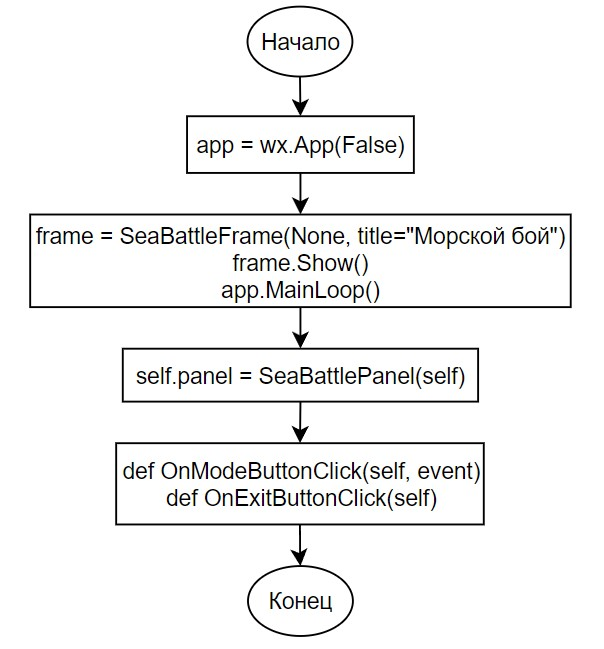
\includegraphics[width = 10cm]{общая.jpg}
\caption{общая блок --- схема.}
\end{figure}

Метод OnModeButtonClick обрабатывает события нажатия кнопок, определяет, какая кнопка была нажата, и запускает соответствующий режим игры. Если ни одна из кнопок режима не была нажата, метод скрывает одну кнопку и показывает другие, обеспечивая правильное расположение кнопок на панели.
Блок --- схема для метода OnModeButtonClick представлена на рисунке 2.2:
\begin{figure}[H]
\graphicspath{ {img/} }
\centering
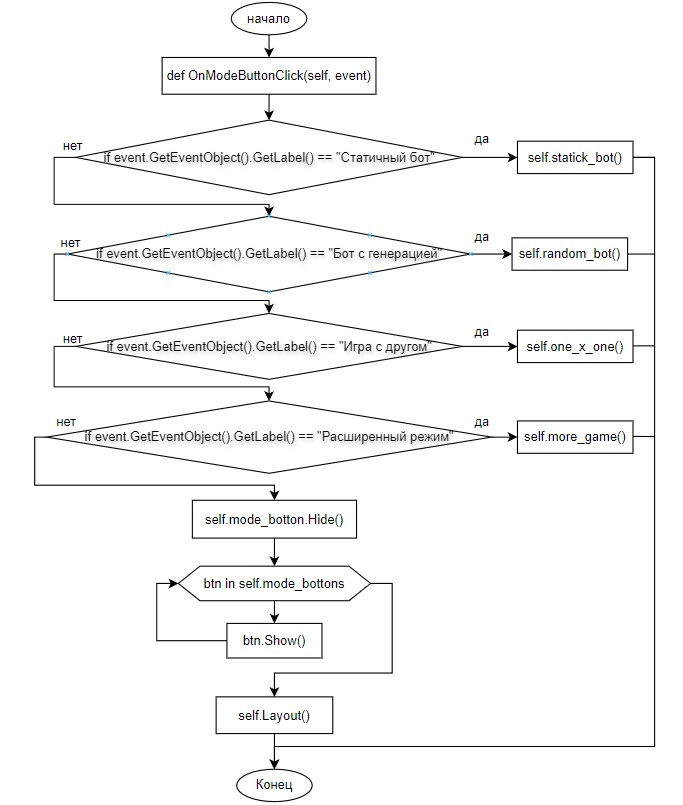
\includegraphics[width = 15cm]{часть.jpg}
\caption{блок --- схема для OnModeButtonClick.}
\end{figure}
\section{\label{sec:ch02/sec07}Тестирование}
При открытии приложения должно создаться окно, в котором находятся две кнопки <<Выбор режима>> и <<Выход>>, на фоне имеется картинка, в менюбаре находятся две доступные кнопки <<Menu>> и <<About>>. Тестирование открытия приложения приведено на рисунке 2.3:
\begin{figure}[H]
\graphicspath{ {img/} }
\centering
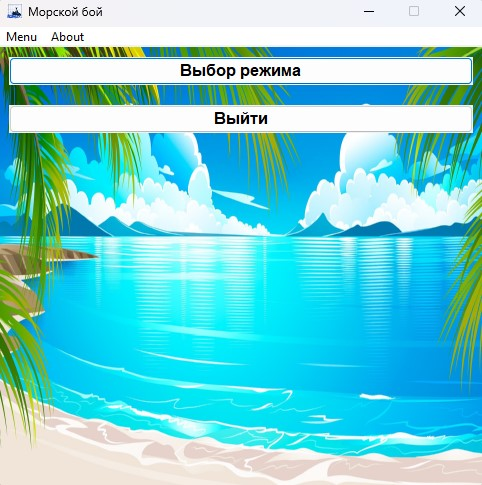
\includegraphics[width = 10cm]{главное окно.jpg}
\caption{Тестирование открытия приложения.}
\end{figure}
При нажатии на кнопку <<Выбор режима>> дополнительно появляются четыре кнопки, с помощью которых запускаются игровые режимы: <<Статический бот>>, <<Бот с генерацией>>, <<Игра с другом>>, <<Расширенный режим>>. Кнопка <<Выбор режима>> пропадает. Тестирование нажатия на кнопку <<Выбор режима>> представлено на рисунке 2.4:
\begin{figure}[H]
\graphicspath{ {img/} }
\centering
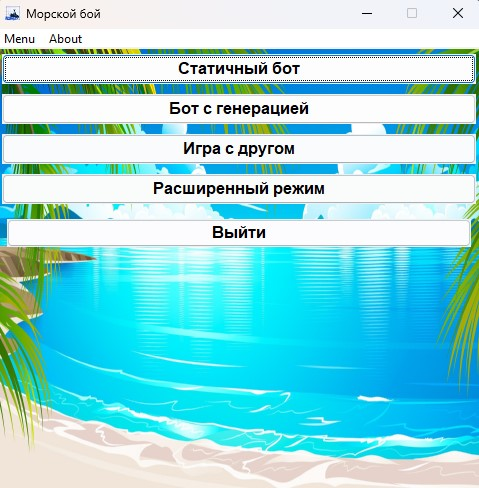
\includegraphics[width = 10cm]{Выбор режима.jpg}
\caption{Тестирование кнопки <<Выбор режима>>.}
\end{figure}
Необходимо проверить возможность постановки корабля вертикально, а после с нажатием кнопки <<Горизонтально>>. Проверка на постановку корабля вертикально представлена на рисунке 2.5:
\begin{figure}[H]
\graphicspath{ {img/} }
\centering
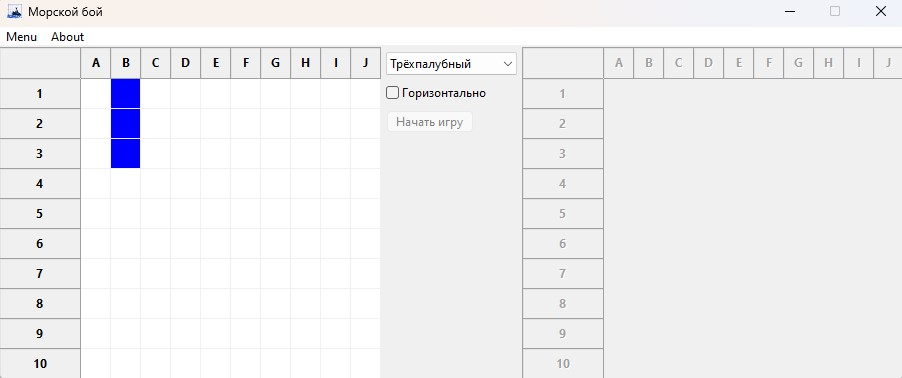
\includegraphics[width = 15cm]{Вертикально.jpg}
\caption{Тестирование на постановку корабля вертикально.}
\end{figure}
Проверка на постановку корабля горизонтально с использованием кнопки <<Горизонтально>> представлена на рисунке 2.6:
\begin{figure}[H]
\graphicspath{ {img/} }
\centering
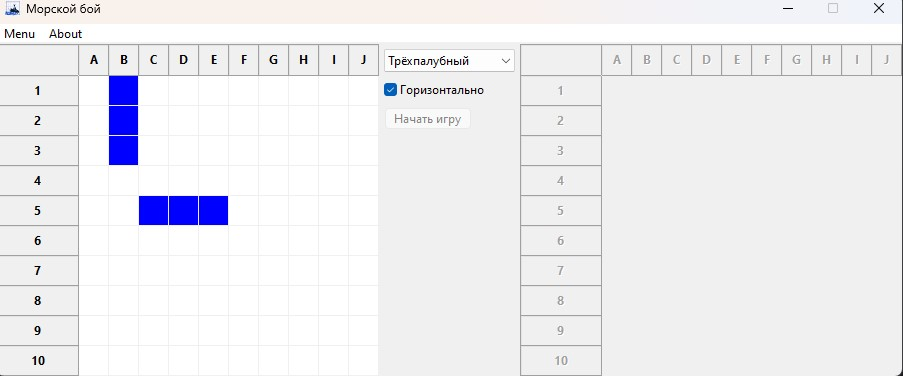
\includegraphics[width = 15cm]{горизонтально.jpg}
\caption{Тестирование на постановку корабля горизонтально.}
\end{figure}
